\newpage
\chapter{Korelační analýza}

Vypočítala jsem korelaci mezi hodnotou shrinkem a tržbami. Jedno pozorování je na agregované na produkt, prodejnu a den záznamu. 
V rámci analýzy jsem srovnávala mezi pouze záznamy produktů, které se vyskytují ve stejné kategorii. Je možné specifikovat úroveň kategorie, na které se analýza spočítá. Dále je třeba určit konkrétní název kategorie.

% https://mathstat.econ.muni.cz/media/12657/pear_cor.pdf
% https://is.muni.cz/www/98951/41610771/43823411/43823458/44159634/44707073/Pavlik_-_Biostatistika_-_kapitola_11.pdf

% úrovně 4, neboť nižší kategorie ve většině případů produkty již dále nedělí, ale pouze specifikují popis kategorie na   

\section{Postup}

Hodnotu shrinku jsem porovnávala s~následujícími ukazateli. 
\begin{itemize}
    \itemsep0em 

    \item Tržby daného produktu.
    \item Tržby daného produktu, které byly v~daný den v~promoakci - ukázalo se, že takové, až na výjimky nejsou.
    \item Součet tržeb všech ostatních produktů v~kategorii.
    \item Součet tržeb všech ostatních produktů v~kategorii, které byly v~daný den v~promoakci.
    \item Součet tržeb všech ostatních produktů v~kategorii, které byly v~daný den v~promoakci nebo byly v~rozmezí jednoho týdne po promoakci.
\end{itemize}

Ke každému ukazateli, jsem ještě vytvořila analogický ukazatel, který uvažoval zpoždění shrinku. V takovém ukazateli, se nebrala hodnota prodeje ze stejného dne, jako byl den záznamu shrinku, ale hodnota z~předchozího dne. Důvodem pro vytvoření takových ukazatelů byla hypotéza, že shrink se může projevit až další den po uskutečněných tržbách. Důvodem může být to, že 

Na základě korelační analýzy je možné roztřídit produkty v~kategorii do tří skupin:
\begin{itemize}
    \itemsep0em 
    \item[] \textbf{Kategorie P} - Produkty, které si samy způsobují shrink.
    \item[] \textbf{Kategorie O} - Produkty, jejichž shrink je způsoben tím, že ostatní produkty v~kategorii jsou v~promoakci.
    \item[] \textbf{Kategorie X} - Produkty, jejichž shrink se nepodařilo vysvětlit pomocí korelační analýzy.
\end{itemize}

Na obrázku \ref*{obr:ctg:g:kategorizace1} je znázorněno rozdělení produktů vzhledem ke korelačnímu koeficientu. 

\begin{figure}[hbtp!]
    \centering
    \captionsetup{justification=centering}
    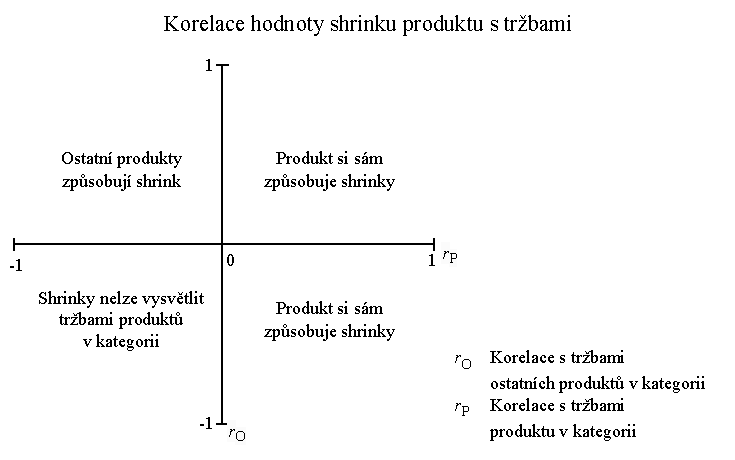
\includegraphics[width=\textwidth]{obrazky/grafy/matice_korelace_typy_DP-graf.pdf}
    \caption{Kategorizace produktů podle korelace hodnoty shrinku produktu s~tržbami.}
    \label{obr:ctg:g:kategorizace1}
\end{figure}

Hypotéza pro zařazení do kategorie P je následující:

Pokud je korelace zaznamenaného shrinku s~tržbami téhož produktu kladná, produkt si způsobuje shrinky sám.
Abych mohla tuto hypotézu potvrdit, nebo vyvrátit, je třeba statisticky otestovat významnost korelačního koeficientu. Formulovala jsem nulovou hypotézu $H_\mathrm{0}$ a alternativní hypotézu $H_\mathrm{A}$ pro koeficient $r_\mathrm{P}$, který měří korelaci mezi hodnotou shrinku a tržbami produktu.
% $$
%     H_\mathrm{0}: r_\mathrm{P} = 0 \qquad \mbox{Výběry nejsou korelované.}  
% $$
% $$   
%     H_\mathrm{A}: r_\mathrm{P} \neq 0 \qquad\mbox{Výběry jsou korelované.}  
% $$
\begin{equation*}
    \begin{aligned}
        H_\mathrm{0}: \quad & r_\mathrm{P} = 0 \qquad \mbox{Výběry nejsou korelované.}  \\
        H_\mathrm{A}: \quad & r_\mathrm{P} \neq 0 \qquad\mbox{Výběry jsou korelované.}\\
    \end{aligned}
\end{equation*}

Hypotéza pro zařazení do kategorie O je následující:

Pokud jsou kladně korelované hodnoty zaznamenaného shrinku a tržby ostatních produktů a zároveň korelace shrinků produktu s~vlastními tržbami je záporná, potom lze vyslovit hypotézu, že shrinky na produktu jsou způsobené ostatními produkty v~promoakci.
Pro toto tvrzení je opět nutné statisticky otestovat koeficienty korelace. Pro koeficient $r_\mathrm{P}$ je statistický test stejný jako v~předchozím případě. Pro koeficient $r_\mathrm{O}$ měřící, jak jsou korelované shrinky a tržby ostatních produktů, je třeba otestovat následující hypotézy.
\begin{equation*}
    \begin{aligned}
        H_\mathrm{0}: \quad & r_\mathrm{O} = 0 \qquad \mbox{Výběry nejsou korelované.}  \\
        H_\mathrm{A}: \quad & r_\mathrm{O} \neq 0 \qquad\mbox{Výběry jsou korelované.}\\
    \end{aligned}
\end{equation*}

Pokud na zvolené hladině významnosti zamítneme nulovou hypotézu pro zkoumané korelační koeficienty, můžeme tvrdit že s~danou pravděpodobností je koeficient statisticky významný. Na základě hodnoty korelace lze pak produkt zařadit do příslušné kategorie. Produkty, u kterých nelze zamítnout, není možné zařadit do tří uvedených kategorií.

Pro výpočet korelačního koeficientu je ještě třeba ověřit předpoklady. Pro Pearsonův korelační koeficient se jedná o~předpoklad normality dat, shodnost rozptylů a nezávislost dat. Pro Spearmanův korelační koeficient jsou předpokládány nezávislé stejně rozdělené náhodné veličiny.

\section{Implementace}

V~této části je uveden přesný postup pro získání kategorizace produktů. Kód je napsaný v~jazyce Python. Součástí kódu je výběr kategorií, které jsou zkoumány, propojení dat shrinků, prodejů a promoakcí, výpočet korelace a ověření předpokladů, statistické testování a rozřazení produktů.

UML diagram pro analýzu.

\subsection{Vstupy a výstupy}

Pro korelační analýzu zaznamenaných shrinků s~tržbami dalších produktů je třeba zajistit data, které se týkají zaznamenaných prodejů, produktů a~prodejen. V~následující části jsou popsány tabulková data, která jsou nezbytná pro správné spuštění analýzy. Dále jsou definované i vstupy, které musí definovat uživatel pro specifikování názvů konkrétních sloupců v~souborech a parametry pro analýzu.

Celkem je požadováno pět vstupních tabulek - záznamy shrinků, záznamy prodejů, záznamy o~promoakcích, číselník produktů s~rozdělením produktové hierarchie. %a~rozdělení prodejen.
Tabulka se zaznamenanými shrinky musí obsahovat sloupec s~datem záznamu, ID produktu, ID prodejny, hodnotu zaznamenaného shrinku. Tabulka s~prodeji potřebuje stejné sloupce jako tabulka se shrinky s~výjimkou že hodnota prodejů je celková prodaná částka, která byla zaznamenaná na dané prodejně v~jeden den u daného produktu. Tabulka s~údaji o promoakcích by měla obsahovat ID produktu, kterého se promoakce týká, začáteční a koncové datum promoakce a ID prodejny, pro kterou promoakce platí.
Všechny záznamové tabulky musí pokrývat stejné časové období. Období může být libovolně dlouhé.
Tabulka produktové hierarchie obsahuje ID produktu, jeho název a libovolně hluboký strom hierarchií. Každá úroveň stromu má vlastní sloupec. Všechny úrovně jsou vyplněné pro každý produkt, tato podmínka je nutná jen pro kategorie, které bude chtít uživatel využít při analýze. 
Tabulka s hierarchie produktů slouží k tomu, aby mohla být napojena na ostatní tabulky a data se pak mohla vyfiltrovat pouze na záznamy týkající se vybrané kategorie.

Před spuštěním hlavní výpočetní části musí uživatel vypsat konkrétní pojmenování sloupců v tabulce do proměnných. Sloupce, které v různých tabulkách označují tytéž hodnoty, musí mít stejný název. V následujícím kódu \ref*{code:colnames} je ukázka zadání. V komentářích je slovní popis o jaký sloupec se jedná. Sloupec by však měl být jasný přímo z názvu proměnné.

\begin{lstlisting}[language=Python, style=mystyle, label={code:colnames}, caption={Definice konkrétních názvů sloupců.}]
product_col      = 'product_id'             # Product ID column
product_name_col = 'name'                   # Product name column
whs_id_col       = 'warehouse_id'           # Store ID column
date_col         = 'date_of_transaction'    # Date of transactions column - for sales and shrinks tables
value_col_shrink = 'cost_value'             # Column with value of shrinks (shrink table)
value_col_sales  = 'cost_value'             # Column with value of total sales (sales table)
promo_col_from   = 'promotion_date_from'    # Starting date of promotion (promotion table)
promo_col_to     = 'promotion_date_to'      # Starting date of promotion (promotion table)
categories       = ['L3','L4','L5','L6', 'name']  # Categories that we want to map to product ID (product hierarchy) 
\end{lstlisting}

Uživatel dále (viz ukázka kódu \ref*{code:params} zadefinuje formát data, který se používá v datumových sloupcích, aby se tyto sloupce mohly převést z~textového řetězce na typ \texttt{datetime}. V~proměnné \texttt{category\_column} je třeba vybrat jednu kategorii (název sloupce). Na této úrovni se poté budou procházet jednotlivé kategorie, v~rámci každé z~nich se pak budou porovnávat a třídit produkty. V dalších proměnných může uživatel změnit umístění tj. název složky, kam se ukládají výsledky kategorizace a grafy. Složky s~těmito názvy se vytvoří jako podsložky aktuální cesty.

\begin{lstlisting}[language=Python,style=mystyle,, label={code:params},  caption={Definice parametrů.}]
date_format = '%Y-%m-%d'                    # Format of date columns
category_column = 'L6'                      # Level od product hierarchy, on which to compare products (have to be in categories)
\end{lstlisting}

\subsection{Popis funkcí a struktura kódu}

Kód pro korelační analýzu je umístěn ve složce \texttt{shrink\_categorization}, struktura složky je vidět na obrázku \ref*{obr:strukturaslozky}.

\begin{figure}[hbtp!]
    \centering
    \captionsetup{justification=centering}
    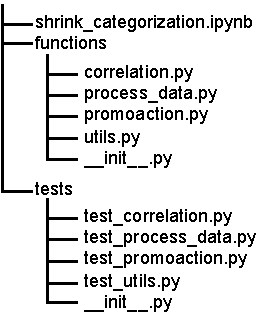
\includegraphics[width=\textwidth]{obrazky/strukturaslozky.pdf}
    \caption{Struktura souborů pro kód zpracovávající korelační analýzu.}
    \label{obr:strukturaslozky}
\end{figure}

Funkce jsou rozčleněny do modulů podle toho, na jaký výpočet jsou zaměřené. Každá funkce má je zdokumentovaná pomocí docstring obsaženého ve své definici. Dokumentace funkce se skládá ze stručného popisu, co funkce dělá, jaké má vstupní parametry a jaký je jejich význam a co funkce vrací. Funkce jsou otestované pomocí unit testů.

Pro práci s tabulkovými daty, které jsou hlavním vstupem, jsem použila balíček \emph{pandas} jazyka Python

\emph{V~závorce je nástin toho, co budu popisovat (TBD)}

\begin{itemize}
    \item Výběr kategorie (Aby se nemuselo zadávat, přesné názvy kategorií systém vybere prvních $n$ nejsilnějších kategorií z~pohledu shrinků.)
    \item Propojení dat
    \item Korelace (Pearsonův, Spearmanův korelační koeficient) (ověření předpokladů (Kolmogorov-Smirnov test pro IID), testování statistické významnosti)
    \item Kategorizace (Nastavení prahu pro velikost korelačního koeficientu)
    \item Pomocné funkce
\end{itemize}

\subsubsection*{Funkce pro vytipování rizikových kategorií}

Funkce \texttt{define\_risk\_categories} vybere prvních $n$ kategorií v~dané produktové hierarchii, kde suma hodnot v dané kategorii, je nejvyšší, resp. nejnižší. Funkce vrací seznam těchto kategorií. Prvním vstupní parametrem je DataFrame, který obsahuje minimálně tři sloupce. Tyto sloupce je třeba definovat jako další parametry funkce. Jedná se o~sloupec \texttt{value\_column}, ve kterém jsou hodnoty, které ohodnocují řádky DataFramu a kategorie. Další sloupec je jedna z~úrovní produktové hierarchie, ve sloupci se nachází názvy, nebo jiné označení, kategorií. Posledním povinným parametrem je počet kategorií, které má funkce vrátit. Dale je funkci možné předat keyword argumenty, které se předají funkci \texttt{sort\_values} z~knihovny \emph{pandas}. Jedná se např. o~parametr pro vzestupné, nebo sestupné řazení. Defaultní řazení je vzestupné, což znamená, že se vezmou kategorie s~nejnižší hodnotou. V této analýze sledujeme vyhozené množství, resp. peníze. Tento ukazatel je záporný, tedy vzestupné řazení vybere ty kategorie, jejichž ztráta byla nejvyšší.

\subsubsection*{Funkce pro výběr pouze dané kategorie ze všech záznamů}
process\_dataframes
select\_category
\subsection{Testování}

Pro testování funkcí jsem použila knihovny \emph(pytest) jazyka Python. Testy lze spustit příkazem \texttt{python -m pytest tests} v kořenovém adresáři projektu - ¨\texttt{shrink\_categorization}. Každý test

\section{Výsledky}
Zvolila jsem 5\% hladinu významnosti pro testování statistické významnosti koeficientů korelace $r_\mathrm{P}$ a $r_\mathrm{O}$.

Nejprve jsem se zaměřila na kategorie z~úrovně 4, a to prvních deset kategorií s~nejvyšší hodnotou shrinků (tj. s~nejvyšší zaznamenanou ztrátou) 

V~tabulce č.~\ref*{tab:kategCorrPorovnani} \emph{(TBD: Bude tam víc kategorii L4.)} jsou porovnání výsledků kategorizace pro kategorii Masné výrobky a Slané pečivo. Měřila jsem postupně korelaci velikosti shrinku s~různými ukazateli pro celkové tržby ostatních produktů. Pro určení míry korelace jsem zvolila Spearmanův korelační koeficient, jelikož data nesplňují předpoklady, které jsou nutné pro použití Pearsonova korelačního koeficientu - data nejsou nezávislá a stejně rozdělená. 
Z uvedených počtů produktů u jednotlivých kategoriích pro různé ukazatele, je patrné, že výsledky se příliš neliší. Pokud bychom se ale zaměřovali na celkové prodeje, nikoli promoční, tak získáváme větší množství produktů, u~nichž nebylo možné vysvětlit shrink pomocí korelace. 

\begin{table}[hbtp!]
    \centering
    \captionsetup{justification=centering}
    \caption{Počet produktů v~kategoriích v~závislosti na různých ukazatelích. Kategorizace proběhla na základě Spearmanova korelačního koeficientu}
    \begin{tabular}{l *{6}{r}}
    \toprule
    \multicolumn{1}{l}{} & \multicolumn{6}{c}{Korelace s~tržbami ostatních produktů} \\
    \multicolumn{1}{l}{} & \multicolumn{2}{c}{Všechny prodeje} & \multicolumn{2}{c}{Prodeje v~promoakci}  & \multicolumn{2}{c}{Prodeje v~a po promoakci} \\
    Kategorie & Stejný den & Další den & Stejný den & Další den & Stejný den & Další den \\
    \midrule
    \multicolumn{7}{c}{Masné výrobky - pultový prodej} \\
    \midrule
    P           & 96   & 96   & 96   & 96   & 96   & 96   \\
    O           & 1     & 1   & 2   & 2   & 2   & 2   \\
    X           & 3     & 3   & 2   & 2   & 2   & 2   \\
    Nevýzn.     & 11    & 11   & 11   & 11   & 11   & 11   \\
    \midrule
    \multicolumn{7}{c}{Slané pečivo} \\
    \midrule
    P           & 131   & 131   & 131   & 131   & 131   & 131   \\
    O           & 9     & 13   & 24   & 24   & 24   & 24   \\
    X           & 16    & 12   & 1    & 1    & 1    & 1    \\
    Nevýzn.     & 90    & 90   & 90   & 90   & 90   & 90   \\
    \bottomrule

    \end{tabular}
    \label{tab:kategCorrPorovnani}
\end{table}



\textbf{Masné výrobky - pultový prodej}

Shrink byl zaznamenaný u 111 produktů v~této kategorii úrovně 4. 96 produktů bylo klasifikováno jako kategorie P, dva jako kategorie O, další dva jako X a u zbylých produktů nebyl koeficient korelace statisticky významný a proto nejde u těchto produktů vyslovit hypotézu pro jejich zařazení.

Produkty, které patří do kategorie O: Velikonoční klobása a Velikonoční česnekový šál - jedná se zcela jistě o sezónní výrobky. \emph{TBD: vyjmenovat i další produkty, keré si způsobují samy, ale je to většina produktů a salámy, šunky, z~kategorie...} 

Dále jsem zkoumala podkategorie Masných výrobků. Porovnávala jsem prodeje v~rámci kategorií na šesté úrovni produktové hierarchie. V~podkategroii Salámy s~krátkou dobou spotřeby se kategorizace potvrdila. Pro kategorii, do níž patří sezónní výrobky - Netučné masné výrobky, nově z~této podkategorie byl jako kategorie O označen i produkt Kladenská pečeně.

\begin{figure}[hbtp!]
    \centering
    \captionsetup{justification=centering}
    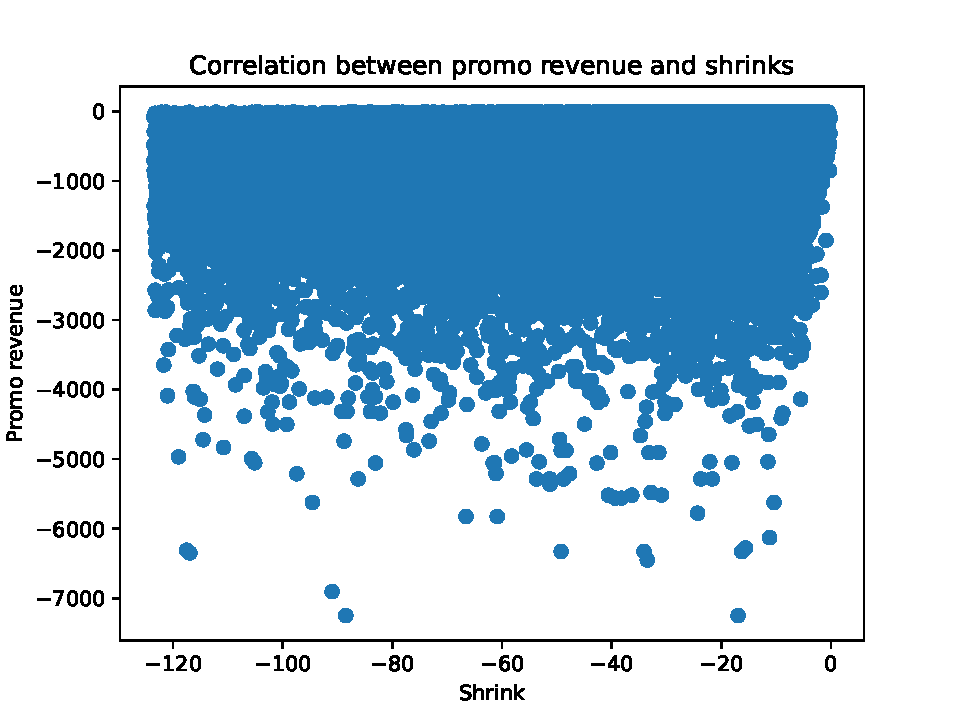
\includegraphics[width=\textwidth]{obrazky/grafy/categorization_charts/categorization_charts_L4_PROC. MEAT SERVICE.pdf}
    \caption{Závislost mezi tržbami produktu a tržbami ostatních produktů v~kategorii během promoakce (Masné výrobky - pultový prodej).}
    \label{obr:ctg:g:graf}
\end{figure}

\textbf{Slané pečivo}

Produkty, které patří do kategorie O:
pletýnka adélka, pletýnka malena, pletýnka sypaná mákem, pletýnka sypaná solí a km., bramborové pečivo s~cibulí, veka cupeko kb, rohlík grahamový aspec, rohlík pivní ora, rohlík staročeský, rohlík obilný mam, rohlík na strouh.karlova, rohl.n str.penam, houska mašek, houska raženka, bageta rust.poh., bageta s~grahamem, bageta chlebová, banketka cereální, dalamánek, kostka cereál malena, ciabatta mini natural, twistr se sýrem a špenatem, anglický rohlík, 

\emph{Nevidím v~této kategorii pravidlo v~tom, co je v~produktech, kterým shrink způsobují ostatní produkty, a které si za to mohou samy. TBD: názvy zobecním...}

\textbf{Sladké pečivo}

čokorolka, závin mák , skořicový vrut, donut bílý se sušnkami, závitek cereální nugátový, rohlík lístový s~ořech. náp, kobliha vanilková šiška, kobliha vanilková v~koš, kobliha s~jablky a skořicí, kobliha s~lísko.náp.a pol, koblih kapsa s~jablky pécé, koláč wellartův, koláč tlač. vícezrnný, koláč šátek makový, koláč s~ovocnou nápl, koláček švestkový , koláček meruňkový , koláček borůvkový, koláč rohový tři náplně , koláč s~makovou náplní, koláč s~tvarohovo nápl, máslový koláč tvaroh, šátek kyn. tvarohová nápl, šáteček s~náplní višňovou , šáteček s~tvaroh.náplní, šátek makový, loupák o., loupák v., loupák m., závin tvaroh , závin kvásk. makový, bavorská hvězdice, makovka pletená mašek, croissant máslový

\textbf{Plodová zelenina}

Shrink byl zaznamenaný u 28 produktů v~této kategorii. 20 produktů bylo klasifikováno jako kategorie P, u zbylých produktů nebyl koeficient korelace statisticky významný a proto nejde u těchto produktů vyslovit hypotézu pro jejich zařazení.


% MEAT
% % \begin{itemize}
% %     \itemsep0em 

% %     \item oboustranná: korelace je nenulová,
% %     \item jednostranná (menší než nula): korelace je záporná
% %     \item jednostranná (větší než nula): korelace je kladná
% % \end{itemize}

% %  MEAT PRODUCTS
% % Catgeorization:  correlation_with_other_products:
% % itself    96
% % False     11
% % None       3
% % other      1
% % Catgeorization:  correlation_with_other_products_past:
% % itself    96
% % False     11
% % None       4
% % Catgeorization:  correlation_with_other_products_promo:
% % itself    96
% % False     11
% % other      2
% % None       2
% % Catgeorization:  correlation_with_other_products_promo_past:
% % itself    96
% % False     11
% % other      2
% None       2

% Analyzing category: SALTY PASTRY of L4 category level.
% ======================================================
% Sizes of dataframes with obly the selected category: 
% Shape of df:  (104427, 22)
% Shape of df:  (8944, 10)
% Shape of df:  (480412, 14)
% Labeling promotions.
% 234020it [01:02, 3733.68it/s]
% Searching for duplicate records.
% 234020it [00:36, 6353.39it/s] 
% Count of rows to drop:  104772
% Shapes of dataframes: Sales:  (477631, 14) Promotions:  (8944, 10) Sales with promo:  (582403, 19) Sales with promo no duplicates:  (477631, 17)
% Calculating  spearman  correlation coefficient.
% Number of products in category:  246

% Products that had no sales during promotion:  223 products.
% Products that had no sales at all:  18 products.
% [22459466, 23194175, 26109718, 27344064, 22095022, 26627342, 21488931, 21976056, 21976124, 22045751, 26627328, 26778808, 25773071, 27735190, 27684436, 27740767, 27710340, 27740750]
% Catgeorization:  correlation_with_other_products:
% itself    131
% False      90
% None       16
% other       9

% Catgeorization:  correlation_with_other_products_past:
% itself    131
% False      90
% None       14
% other      11

% Catgeorization:  correlation_with_other_products_promo:
% itself    131
% False      90
% other      24
% None        1

% Catgeorization:  correlation_with_other_products_promo_past:
% itself    131
% False      90
% other      24
% None        1

% Analyzing category: FRUIT VEGETABLE of L4 category level.
% =========================================================
% Sizes of dataframes with obly the selected category: 
% Shape of df:  (34680, 22)
% Shape of df:  (5556, 10)
% Shape of df:  (179351, 14)
% Labeling promotions.
% 114262it [00:30, 3747.84it/s]
% Searching for duplicate records.
% 114262it [00:13, 8487.78it/s] 
% Count of rows to drop:  49439
% Shapes of dataframes: Sales:  (177703, 14) Promotions:  (5556, 10) Sales with promo:  (227142, 19) Sales with promo no duplicates:  (177703, 17)
% Calculating  spearman  correlation coefficient.
% Number of products in category:  28

% Products that had no sales during promotion:  16 products.
% [20444853, 20445836, 20698171, 26398969, 24363303, 20452094, 20445553, 21497513, 20446086, 27299395, 24228862, 24391078, 26977775, 23930742, 27227947, 27333501]
% Products that had no sales at all:  1 products.
% [27333501]
% Catgeorization:  correlation_with_other_products:
% itself    20
% False      8

% Catgeorization:  correlation_with_other_products_past:
% itself    20
% False      8

% Catgeorization:  correlation_with_other_products_promo:
% itself    20
% False      8

% Catgeorization:  correlation_with_other_products_promo_past:
% itself    20
% False      8

% Analyzing category: SWEET PASTRY of L4 category level.
% ======================================================
% Sizes of dataframes with obly the selected category: 
% Shape of df:  (48701, 22)
% Shape of df:  (16131, 10)
% Shape of df:  (634294, 14)
% Labeling promotions.
% 304122it [01:18, 3892.35it/s]
% Searching for duplicate records.
% 304122it [00:41, 7351.05it/s]
% Count of rows to drop:  24675
% Shapes of dataframes: Sales:  (632724, 14) Promotions:  (16131, 10) Sales with promo:  (657399, 19) Sales with promo no duplicates:  (632724, 17)
% Calculating  spearman  correlation coefficient.
% Number of products in category:  386

% Products that had no sales during promotion:  331 products.
% Products that had no sales at all:  10 products.
% [22055101, 27729915, 26159140, 26778860, 21976186, 26778846, 27738740, 27737170, 21976209, 27636015]
% Catgeorization:  correlation_with_other_products:
% False     197
% itself    155
% None       34

% Catgeorization:  correlation_with_other_products_past:
% False     197
% itself    155
% None       30
% other       4

% Catgeorization:  correlation_with_other_products_promo:
% False     197
% itself    155
% other      34

% Catgeorization:  correlation_with_other_products_promo_past:
% False     197
% itself    155
% other      34

% Analyzing category: RED MEAT of L4 category level.
% ==================================================
% Sizes of dataframes with obly the selected category: 
% Shape of df:  (17391, 22)
% Shape of df:  (29066, 10)
% Shape of df:  (332815, 14)
% Labeling promotions.
% 390190it [01:35, 4092.89it/s]
% Searching for duplicate records.
% 390190it [00:50, 7735.99it/s] 
% Count of rows to drop:  174298

% Products that had no sales during promotion:  65 products.
% [24293174, 24560115, 25720938, 24125499, 27725788, 24646864, 26040561, 26042824, 22840400, 26044910, 26566849, 26123615, 26130309, 26045061, 26045016, 27669778, 26045030, 26159881, 27166031, 22840387, 25881493, 26123677, 22257628, 26045115, 26124872, 26915975, 25960051, 26044811, 27712375, 25615036, 26872667, 26277202, 26770987, 26725192, 26044927, 26277226, 26177038, 27712399, 26044989, 27557235, 26770901, 27522660, 26643885, 26771007, 26771120, 27133279, 26157870, 26125275, 27743164, 26835846, 26871677, 26157733, 27102176, 26954905, 27260081, 27098868, 27103715, 27260265, 27738474, 27100912, 27425893, 27738481, 26566856, 27743157, 26771137]
% Products that had no sales at all:  17 products.
% [27725788, 26123615, 26130309, 26159881, 27166031, 26123677, 26124872, 26044989, 27133279, 26125275, 27743164, 26157733, 27098868, 27103715, 27738474, 27738481, 27743157]
% Catgeorization:  correlation_with_other_products:
% itself    96
% False     39
% None       3


% Catgeorization:  correlation_with_other_products_past:
% itself    96
% False     39
% None       3


% Catgeorization:  correlation_with_other_products_promo:
% itself    96
% False     39
% other      3


% Catgeorization:  correlation_with_other_products_promo_past:
% itself    96
% False     39
% other      3

% % https://docs.scipy.org/doc/scipy/reference/generated/scipy.stats.spearmanr.html
% % https://statistics.laerd.com/statistical-guides/spearmans-rank-order-correlation-statistical-guide-2.php There is no [monotonic] association between the two variables [in the population].






% Analyzing category: PROC. MEAT SERVICE of L4 category level.
% ============================================================
% Sizes of dataframes with obly the selected category: 
% Shape of df:  (303847, 22)
% Shape of df:  (70584, 10)
% Shape of df:  (555853, 14)
% Labeling promotions.
% 1679273it [08:33, 3270.31it/s]
% Searching for duplicate records.
% 1679273it [04:13, 6615.74it/s]
% Count of rows to drop:  1165224
% Shapes of dataframes: Sales:  (554305, 14) Promotions:  (70584, 10) Sales with promo:  (1719529, 19) Sales with promo no duplicates:  (554305, 17)
% Method:  pearson  after promo:  False
% Calculating  pearson  correlation coefficient.
% Number of products in category:  111

% Products that had no sales during promotion:  40 products.
% [20454081, 20454111, 25666854, 25961225, 26872896, 23180666, 20453978, 23373204, 24888967, 25478198, 25726787, 25961164, 26831718, 26831817, 27254783, 27571781, 27627761, 25726299, 25961140, 27150054, 25726046, 25726015, 25842371, 27571774, 20402082, 26835587, 25959000, 27722930, 27571798, 27736982, 27254486, 25726060, 27739174, 27737033, 27738504, 26835624, 27738733, 27611357, 25842579, 26831824]
% Products that had no sales at all:  6 products.
% [27722930, 27736982, 27739174, 27737033, 27738504, 27738733]
% Method:  pearson  after promo:  False
% Catgeorization:  correlation_with_other_products:
% itself    100
% False       9
% None        2


% Catgeorization:  correlation_with_other_products_past:
% itself    100
% False       9
% None        2


% Catgeorization:  correlation_with_other_products_promo:
% itself    100
% False       9
% other       1
% None        1


% Catgeorization:  correlation_with_other_products_promo_past:
% itself    100
% False       9
% other       1
% None        1


% Method:  spearman  after promo:  False
% Calculating  spearman  correlation coefficient.
% Number of products in category:  111
% Products that had no sales during promotion:  40 products.
% [20454081, 20454111, 25666854, 25961225, 26872896, 23180666, 20453978, 23373204, 24888967, 25478198, 25726787, 25961164, 26831718, 26831817, 27254783, 27571781, 27627761, 25726299, 25961140, 27150054, 25726046, 25726015, 25842371, 27571774, 20402082, 26835587, 25959000, 27722930, 27571798, 27736982, 27254486, 25726060, 27739174, 27737033, 27738504, 26835624, 27738733, 27611357, 25842579, 26831824]
% Products that had no sales at all:  6 products.
% [27722930, 27736982, 27739174, 27737033, 27738504, 27738733]
% Method:  spearman  after promo:  False
% Catgeorization:  correlation_with_other_products:
% itself    96
% False     11
% None       3
% other      1


% Catgeorization:  correlation_with_other_products_past:
% itself    96
% False     11
% None       3
% other      1


% Catgeorization:  correlation_with_other_products_promo:
% itself    96
% False     11
% other      2
% None       2


% Catgeorization:  correlation_with_other_products_promo_past:
% itself    96
% False     11
% other      2
% None       2


% Method:  pearson  after promo:  True
% Calculating  pearson  correlation coefficient.
% Number of products in category:  111
% Products that had no sales during promotion:  32 products.
% [26872896, 24888967, 25478198, 25726787, 25961164, 26831718, 26831817, 27254783, 27571781, 27627761, 25726299, 25961140, 27150054, 25726046, 25726015, 27571774, 20402082, 26835587, 25959000, 27722930, 27571798, 27736982, 27254486, 25726060, 27739174, 27737033, 27738504, 26835624, 27738733, 27611357, 25842579, 26831824]
% Products that had no sales at all:  6 products.
% [27722930, 27736982, 27739174, 27737033, 27738504, 27738733]
% Method:  pearson  after promo:  True
% Catgeorization:  correlation_with_other_products:
% itself    100
% False       9
% None        2


% Catgeorization:  correlation_with_other_products_past:
% itself    100
% False       9
% None        2


% Catgeorization:  correlation_with_other_products_promo:
% itself    100
% False       9
% other       1
% None        1


% Catgeorization:  correlation_with_other_products_promo_past:
% itself    100
% False       9
% other       1
% None        1


% Method:  spearman  after promo:  True
% Calculating  spearman  correlation coefficient.
% Number of products in category:  111
% Products that had no sales during promotion:  32 products.
% [26872896, 24888967, 25478198, 25726787, 25961164, 26831718, 26831817, 27254783, 27571781, 27627761, 25726299, 25961140, 27150054, 25726046, 25726015, 27571774, 20402082, 26835587, 25959000, 27722930, 27571798, 27736982, 27254486, 25726060, 27739174, 27737033, 27738504, 26835624, 27738733, 27611357, 25842579, 26831824]
% Products that had no sales at all:  6 products.
% [27722930, 27736982, 27739174, 27737033, 27738504, 27738733]
% Method:  spearman  after promo:  True
% Catgeorization:  correlation_with_other_products:
% itself    96
% False     11
% None       4


% Catgeorization:  correlation_with_other_products_past:
% itself    96
% False     11
% None       4


% Catgeorization:  correlation_with_other_products_promo:
% itself    96
% False     11
% other      2
% None       2


% Catgeorization:  correlation_with_other_products_promo_past:
% itself    96
% False     11
% other      2
% None       2


% Analyzing category: SALTY PASTRY of L4 category level.
% ======================================================
% Sizes of dataframes with obly the selected category: 
% Shape of df:  (104427, 22)
% Shape of df:  (8944, 10)
% Shape of df:  (480412, 14)
% Labeling promotions.
% 234020it [01:11, 3260.33it/s]
% Searching for duplicate records.
% 234020it [00:30, 7668.35it/s] 
% Count of rows to drop:  104772
% Shapes of dataframes: Sales:  (477631, 14) Promotions:  (8944, 10) Sales with promo:  (582403, 19) Sales with promo no duplicates:  (477631, 17)
% Method:  pearson  after promo:  False
% Calculating  pearson  correlation coefficient.
% Number of products in category:  246
% Products that had no sales during promotion:  227 products.
% [20428587, 20480905, 21852039, 23472266, 25467697, 27422731, 27442449, 27456934, 27516850, 27516867, 27544884, 27544907, 27544952, 27544983, 27578025, 27609699, 25672985, 26782034, 27544914, 27544938, 23472259, 27123195, 27544877, 27544891, 27603581, 25310863, 26576442, 26627373, 27123201, 27274750, 27574270, 22459466, 23194175, 23549074, 25895667, 26109718, 26737430, 26737461, 26737478, 27266038, 27269244, 27344064, 27603598, 27619810, 22095022, 26627342, 27638019, 20783808, 21488931, 21976056, 21976124, 22045751, 26627328, 26709468, 27442760, 27312759, 26737539, 26778808, 21471971, 24587136, 27544969, 25318074, 25322194, 25892369, 26960975, 25512700, 23319905, 25673005, 23635739, 25516234, 26359205, 25012200, 25175639, 25431483, 25430783, 25430837, 25430820, 25773071, 27075234, 27075227, 25629620, 26571362, 26571324, 26571331, 27601532, 26786698, 27710418, 22941404, 25504422, 27034071, 26975085, 27449943, 25548761, 25663075, 27195000, 24744881, 27641569, 26445540, 27201930, 22957733, 27374993, 22962294, 25426496, 25426502, 25254792, 27610640, 25506242, 26546117, 27610664, 27735190, 25507294, 25507256, 25506297, 25506303, 22993847, 22993885, 25504439, 25504460, 25571608, 25431599, 27329290, 21482922, 24174381, 25390261, 25390254, 25390643, 25394368, 24328579, 25665864, 24644167, 27329269, 25594836, 22933904, 22933973, 27619513, 27384039, 27384053, 25393422, 25891966, 27134641, 27134634, 23549067, 27152706, 25665802, 25605327, 26787008, 25630602, 26035062, 27455630, 25504446, 27620175, 25571615, 25571660, 27134658, 27134665, 27134689, 24323611, 25498554, 25630596, 25630619, 27619520, 26802046, 27134719, 26975740, 27603611, 25513318, 27282670, 27696729, 27466261, 22993892, 22662200, 25630466, 22019943, 27712306, 27684436, 27278116, 26381350, 26885506, 27307656, 26389400, 27329139, 22516657, 27329184, 27329115, 27032404, 27215937, 26386973, 27453179, 27715444, 25756999, 27128473, 26347394, 27136768, 25661224, 24277365, 25048698, 26434582, 27152492, 27715451, 23478992, 26975078, 26391175, 26802060, 25326185, 26381459, 26576848, 24644143, 25605273, 25066159, 25630657, 26581798, 27574225, 26975689, 27620182, 26381381, 24704427, 26975764, 24644150, 22126221, 25504491, 27710432, 27740767, 27710340, 26502755, 27312827, 27740750, 26579221]
% Products that had no sales at all:  18 products.
% [22459466, 23194175, 26109718, 27344064, 22095022, 26627342, 21488931, 21976056, 21976124, 22045751, 26627328, 26778808, 25773071, 27735190, 27684436, 27740767, 27710340, 27740750]
% Method:  pearson  after promo:  False
% Catgeorization:  correlation_with_other_products:
% itself    130
% False     100
% None       13
% other       3


% Catgeorization:  correlation_with_other_products_past:
% itself    130
% False     100
% None       11
% other       5


% Catgeorization:  correlation_with_other_products_promo:
% itself    130
% False     100
% other      16


% Catgeorization:  correlation_with_other_products_promo_past:
% itself    130
% False     100
% other      16


% Method:  spearman  after promo:  False
% Calculating  spearman  correlation coefficient.
% Number of products in category:  246
% Products that had no sales during promotion:  227 products.
% [20428587, 20480905, 21852039, 23472266, 25467697, 27422731, 27442449, 27456934, 27516850, 27516867, 27544884, 27544907, 27544952, 27544983, 27578025, 27609699, 25672985, 26782034, 27544914, 27544938, 23472259, 27123195, 27544877, 27544891, 27603581, 25310863, 26576442, 26627373, 27123201, 27274750, 27574270, 22459466, 23194175, 23549074, 25895667, 26109718, 26737430, 26737461, 26737478, 27266038, 27269244, 27344064, 27603598, 27619810, 22095022, 26627342, 27638019, 20783808, 21488931, 21976056, 21976124, 22045751, 26627328, 26709468, 27442760, 27312759, 26737539, 26778808, 21471971, 24587136, 27544969, 25318074, 25322194, 25892369, 26960975, 25512700, 23319905, 25673005, 23635739, 25516234, 26359205, 25012200, 25175639, 25431483, 25430783, 25430837, 25430820, 25773071, 27075234, 27075227, 25629620, 26571362, 26571324, 26571331, 27601532, 26786698, 27710418, 22941404, 25504422, 27034071, 26975085, 27449943, 25548761, 25663075, 27195000, 24744881, 27641569, 26445540, 27201930, 22957733, 27374993, 22962294, 25426496, 25426502, 25254792, 27610640, 25506242, 26546117, 27610664, 27735190, 25507294, 25507256, 25506297, 25506303, 22993847, 22993885, 25504439, 25504460, 25571608, 25431599, 27329290, 21482922, 24174381, 25390261, 25390254, 25390643, 25394368, 24328579, 25665864, 24644167, 27329269, 25594836, 22933904, 22933973, 27619513, 27384039, 27384053, 25393422, 25891966, 27134641, 27134634, 23549067, 27152706, 25665802, 25605327, 26787008, 25630602, 26035062, 27455630, 25504446, 27620175, 25571615, 25571660, 27134658, 27134665, 27134689, 24323611, 25498554, 25630596, 25630619, 27619520, 26802046, 27134719, 26975740, 27603611, 25513318, 27282670, 27696729, 27466261, 22993892, 22662200, 25630466, 22019943, 27712306, 27684436, 27278116, 26381350, 26885506, 27307656, 26389400, 27329139, 22516657, 27329184, 27329115, 27032404, 27215937, 26386973, 27453179, 27715444, 25756999, 27128473, 26347394, 27136768, 25661224, 24277365, 25048698, 26434582, 27152492, 27715451, 23478992, 26975078, 26391175, 26802060, 25326185, 26381459, 26576848, 24644143, 25605273, 25066159, 25630657, 26581798, 27574225, 26975689, 27620182, 26381381, 24704427, 26975764, 24644150, 22126221, 25504491, 27710432, 27740767, 27710340, 26502755, 27312827, 27740750, 26579221]
% Products that had no sales at all:  18 products.
% [22459466, 23194175, 26109718, 27344064, 22095022, 26627342, 21488931, 21976056, 21976124, 22045751, 26627328, 26778808, 25773071, 27735190, 27684436, 27740767, 27710340, 27740750]
% Method:  spearman  after promo:  False
% Catgeorization:  correlation_with_other_products:
% itself    131
% False      90
% None       16
% other       9


% Catgeorization:  correlation_with_other_products_past:
% itself    131
% False      90
% other      13
% None       12


% Catgeorization:  correlation_with_other_products_promo:
% itself    131
% False      90
% other      24
% None        1


% Catgeorization:  correlation_with_other_products_promo_past:
% itself    131
% False      90
% other      24
% None        1


% Method:  pearson  after promo:  True
% Calculating  pearson  correlation coefficient.
% Number of products in category:  246
% 246it [01:23,  2.93it/s]
% Products that had no sales during promotion:  223 products.
% [20428587, 20480905, 21852039, 23472266, 25467697, 27442449, 27456934, 27516850, 27516867, 27544884, 27544907, 27544952, 27544983, 27578025, 27609699, 25672985, 26782034, 27544914, 27544938, 23472259, 27123195, 27544877, 27544891, 25310863, 26576442, 26627373, 27123201, 27274750, 27574270, 22459466, 23194175, 23549074, 25895667, 26109718, 26737430, 26737461, 26737478, 27266038, 27269244, 27344064, 27619810, 22095022, 26627342, 27638019, 20783808, 21488931, 21976056, 21976124, 22045751, 26627328, 26709468, 27442760, 27312759, 26737539, 26778808, 21471971, 24587136, 27544969, 25318074, 25322194, 25892369, 25512700, 23319905, 25673005, 23635739, 25516234, 26359205, 25012200, 25175639, 25431483, 25430783, 25430837, 25430820, 25773071, 27075234, 27075227, 25629620, 26571362, 26571324, 26571331, 27601532, 26786698, 27710418, 22941404, 25504422, 27034071, 26975085, 27449943, 25548761, 25663075, 27195000, 24744881, 27641569, 26445540, 27201930, 22957733, 27374993, 22962294, 25426496, 25426502, 25254792, 27610640, 25506242, 26546117, 27610664, 27735190, 25507294, 25507256, 25506297, 25506303, 22993847, 22993885, 25504439, 25504460, 25571608, 25431599, 27329290, 21482922, 24174381, 25390261, 25390254, 25390643, 25394368, 24328579, 25665864, 24644167, 27329269, 25594836, 22933904, 22933973, 27619513, 27384039, 27384053, 25393422, 25891966, 27134641, 27134634, 23549067, 27152706, 25665802, 25605327, 26787008, 25630602, 26035062, 27455630, 25504446, 27620175, 25571615, 25571660, 27134658, 27134665, 27134689, 24323611, 25498554, 25630596, 25630619, 27619520, 26802046, 27134719, 26975740, 27603611, 25513318, 27282670, 27696729, 27466261, 22993892, 22662200, 25630466, 22019943, 27712306, 27684436, 27278116, 26381350, 26885506, 27307656, 26389400, 27329139, 22516657, 27329184, 27329115, 27032404, 27215937, 26386973, 27453179, 27715444, 25756999, 27128473, 26347394, 27136768, 25661224, 24277365, 25048698, 26434582, 27152492, 27715451, 23478992, 26975078, 26391175, 26802060, 25326185, 26381459, 26576848, 24644143, 25605273, 25066159, 25630657, 26581798, 27574225, 26975689, 27620182, 26381381, 24704427, 26975764, 24644150, 22126221, 25504491, 27710432, 27740767, 27710340, 26502755, 27312827, 27740750, 26579221]
% Products that had no sales at all:  18 products.
% [22459466, 23194175, 26109718, 27344064, 22095022, 26627342, 21488931, 21976056, 21976124, 22045751, 26627328, 26778808, 25773071, 27735190, 27684436, 27740767, 27710340, 27740750]
% Method:  pearson  after promo:  True
% Catgeorization:  correlation_with_other_products:
% itself    130
% False     100
% None       14
% other       2


% Catgeorization:  correlation_with_other_products_past:
% itself    130
% False     100
% None       13
% other       3


% Catgeorization:  correlation_with_other_products_promo:
% itself    130
% False     100
% other      16


% Catgeorization:  correlation_with_other_products_promo_past:
% itself    130
% False     100
% other      16


% Method:  spearman  after promo:  True
% Products that had no sales during promotion:  223 products.
% [20428587, 20480905, 21852039, 23472266, 25467697, 27442449, 27456934, 27516850, 27516867, 27544884, 27544907, 27544952, 27544983, 27578025, 27609699, 25672985, 26782034, 27544914, 27544938, 23472259, 27123195, 27544877, 27544891, 25310863, 26576442, 26627373, 27123201, 27274750, 27574270, 22459466, 23194175, 23549074, 25895667, 26109718, 26737430, 26737461, 26737478, 27266038, 27269244, 27344064, 27619810, 22095022, 26627342, 27638019, 20783808, 21488931, 21976056, 21976124, 22045751, 26627328, 26709468, 27442760, 27312759, 26737539, 26778808, 21471971, 24587136, 27544969, 25318074, 25322194, 25892369, 25512700, 23319905, 25673005, 23635739, 25516234, 26359205, 25012200, 25175639, 25431483, 25430783, 25430837, 25430820, 25773071, 27075234, 27075227, 25629620, 26571362, 26571324, 26571331, 27601532, 26786698, 27710418, 22941404, 25504422, 27034071, 26975085, 27449943, 25548761, 25663075, 27195000, 24744881, 27641569, 26445540, 27201930, 22957733, 27374993, 22962294, 25426496, 25426502, 25254792, 27610640, 25506242, 26546117, 27610664, 27735190, 25507294, 25507256, 25506297, 25506303, 22993847, 22993885, 25504439, 25504460, 25571608, 25431599, 27329290, 21482922, 24174381, 25390261, 25390254, 25390643, 25394368, 24328579, 25665864, 24644167, 27329269, 25594836, 22933904, 22933973, 27619513, 27384039, 27384053, 25393422, 25891966, 27134641, 27134634, 23549067, 27152706, 25665802, 25605327, 26787008, 25630602, 26035062, 27455630, 25504446, 27620175, 25571615, 25571660, 27134658, 27134665, 27134689, 24323611, 25498554, 25630596, 25630619, 27619520, 26802046, 27134719, 26975740, 27603611, 25513318, 27282670, 27696729, 27466261, 22993892, 22662200, 25630466, 22019943, 27712306, 27684436, 27278116, 26381350, 26885506, 27307656, 26389400, 27329139, 22516657, 27329184, 27329115, 27032404, 27215937, 26386973, 27453179, 27715444, 25756999, 27128473, 26347394, 27136768, 25661224, 24277365, 25048698, 26434582, 27152492, 27715451, 23478992, 26975078, 26391175, 26802060, 25326185, 26381459, 26576848, 24644143, 25605273, 25066159, 25630657, 26581798, 27574225, 26975689, 27620182, 26381381, 24704427, 26975764, 24644150, 22126221, 25504491, 27710432, 27740767, 27710340, 26502755, 27312827, 27740750, 26579221]
% Products that had no sales at all:  18 products.
% [22459466, 23194175, 26109718, 27344064, 22095022, 26627342, 21488931, 21976056, 21976124, 22045751, 26627328, 26778808, 25773071, 27735190, 27684436, 27740767, 27710340, 27740750]
% Method:  spearman  after promo:  True
% Catgeorization:  correlation_with_other_products:
% itself    131
% False      90
% None       16
% other       9


% Catgeorization:  correlation_with_other_products_past:
% itself    131
% False      90
% None       14
% other      11


% Catgeorization:  correlation_with_other_products_promo:
% itself    131
% False      90
% other      24
% None        1


% Catgeorization:  correlation_with_other_products_promo_past:
% itself    131
% False      90
% other      24
% None        1


% ./categorization_charts/categorization_charts_L4_SALTY PASTRY.pdf
% Analyzing category: FRUIT VEGETABLE of L4 category level.
% =========================================================
% Sizes of dataframes with obly the selected category: 
% Shape of df:  (34680, 22)
% Shape of df:  (5556, 10)
% Shape of df:  (179351, 14)
% Labeling promotions.
% 114262it [00:29, 3873.93it/s]
% Searching for duplicate records.
% 114262it [00:14, 8118.47it/s]
% Count of rows to drop:  49439
% Shapes of dataframes: Sales:  (177703, 14) Promotions:  (5556, 10) Sales with promo:  (227142, 19) Sales with promo no duplicates:  (177703, 17)
% Method:  pearson  after promo:  False
% Calculating  pearson  correlation coefficient.
% Number of products in category:  28

% Products that had no sales during promotion:  17 products.
% [20444853, 20445836, 20698171, 26398969, 24363303, 20452094, 20445553, 21497513, 20446086, 27299395, 24228862, 24391078, 27186244, 26977775, 23930742, 27227947, 27333501]
% Products that had no sales at all:  1 products.
% [27333501]
% Method:  pearson  after promo:  False
% Catgeorization:  correlation_with_other_products:
% itself    23
% False      5


% Catgeorization:  correlation_with_other_products_past:
% itself    23
% False      5


% Catgeorization:  correlation_with_other_products_promo:
% itself    23
% False      5


% Catgeorization:  correlation_with_other_products_promo_past:
% itself    23
% False      5


% Method:  spearman  after promo:  False
% Calculating  spearman  correlation coefficient.
% Number of products in category:  28

% Products that had no sales during promotion:  17 products.
% [20444853, 20445836, 20698171, 26398969, 24363303, 20452094, 20445553, 21497513, 20446086, 27299395, 24228862, 24391078, 27186244, 26977775, 23930742, 27227947, 27333501]
% Products that had no sales at all:  1 products.
% [27333501]
% Method:  spearman  after promo:  False
% Catgeorization:  correlation_with_other_products:
% itself    20
% False      8


% Catgeorization:  correlation_with_other_products_past:
% itself    20
% False      8


% Catgeorization:  correlation_with_other_products_promo:
% itself    20
% False      8


% Catgeorization:  correlation_with_other_products_promo_past:
% itself    20
% False      8


% Method:  pearson  after promo:  True
% Calculating  pearson  correlation coefficient.
% Number of products in category:  28

% Products that had no sales during promotion:  16 products.
% [20444853, 20445836, 20698171, 26398969, 24363303, 20452094, 20445553, 21497513, 20446086, 27299395, 24228862, 24391078, 26977775, 23930742, 27227947, 27333501]
% Products that had no sales at all:  1 products.
% [27333501]
% Method:  pearson  after promo:  True
% Catgeorization:  correlation_with_other_products:
% itself    23
% False      5


% Catgeorization:  correlation_with_other_products_past:
% itself    23
% False      5


% Catgeorization:  correlation_with_other_products_promo:
% itself    23
% False      5


% Catgeorization:  correlation_with_other_products_promo_past:
% itself    23
% False      5


% Method:  spearman  after promo:  True
% Calculating  spearman  correlation coefficient.
% Number of products in category:  28

% Products that had no sales during promotion:  16 products.
% [20444853, 20445836, 20698171, 26398969, 24363303, 20452094, 20445553, 21497513, 20446086, 27299395, 24228862, 24391078, 26977775, 23930742, 27227947, 27333501]
% Products that had no sales at all:  1 products.
% [27333501]
% Method:  spearman  after promo:  True
% Catgeorization:  correlation_with_other_products:
% itself    20
% False      8


% Catgeorization:  correlation_with_other_products_past:
% itself    20
% False      8


% Catgeorization:  correlation_with_other_products_promo:
% itself    20
% False      8


% Catgeorization:  correlation_with_other_products_promo_past:
% itself    20
% False      8


% ./categorization_charts/categorization_charts_L4_FRUIT VEGETABLE.pdf
% Analyzing category: SWEET PASTRY of L4 category level.
% ======================================================
% Sizes of dataframes with obly the selected category: 
% Shape of df:  (48701, 22)
% Shape of df:  (16131, 10)
% Shape of df:  (634294, 14)
% Labeling promotions.
% 304122it [01:10, 4326.14it/s]
% Searching for duplicate records.
% 304122it [00:43, 6952.49it/s]
% Count of rows to drop:  24675
% Shapes of dataframes: Sales:  (632724, 14) Promotions:  (16131, 10) Sales with promo:  (657399, 19) Sales with promo no duplicates:  (632724, 17)
% Method:  pearson  after promo:  False
% Calculating  pearson  correlation coefficient.
% Number of products in category:  386

% Products that had no sales during promotion:  339 products.

% Products that had no sales at all:  10 products.
% [22055101, 27729915, 26159140, 26778860, 21976186, 26778846, 27738740, 27737170, 21976209, 27636015]
% Method:  pearson  after promo:  False
% Catgeorization:  correlation_with_other_products:
% False     228
% itself    143
% None       15


% Catgeorization:  correlation_with_other_products_past:
% False     228
% itself    143
% None       15


% Catgeorization:  correlation_with_other_products_promo:
% False     228
% itself    143
% other      15


% Catgeorization:  correlation_with_other_products_promo_past:
% False     228
% itself    143
% other      15


% Method:  spearman  after promo:  False
% Calculating  spearman  correlation coefficient.
% Number of products in category:  386

% Products that had no sales at all:  10 products.
% [22055101, 27729915, 26159140, 26778860, 21976186, 26778846, 27738740, 27737170, 21976209, 27636015]
% Method:  spearman  after promo:  False
% Catgeorization:  correlation_with_other_products:
% False     197
% itself    155
% None       34


% Catgeorization:  correlation_with_other_products_past:
% False     197
% itself    155
% None       31
% other       3


% Catgeorization:  correlation_with_other_products_promo:
% False     197
% itself    155
% other      34


% Catgeorization:  correlation_with_other_products_promo_past:
% False     197
% itself    155
% other      34


% Method:  pearson  after promo:  True
% Calculating  pearson  correlation coefficient.
% Number of products in category:  386

% Products that had no sales at all:  10 products.
% [22055101, 27729915, 26159140, 26778860, 21976186, 26778846, 27738740, 27737170, 21976209, 27636015]
% Method:  pearson  after promo:  True
% Catgeorization:  correlation_with_other_products:
% False     228
% itself    143
% None       15


% Catgeorization:  correlation_with_other_products_past:
% False     228
% itself    143
% None       15


% Catgeorization:  correlation_with_other_products_promo:
% False     228
% itself    143
% other      15


% Catgeorization:  correlation_with_other_products_promo_past:
% False     228
% itself    143
% other      15


% Method:  spearman  after promo:  True
% Calculating  spearman  correlation coefficient.
% Number of products in category:  386
% Method:  spearman  after promo:  True
% Catgeorization:  correlation_with_other_products:
% False     197
% itself    155
% None       34


% Catgeorization:  correlation_with_other_products_past:
% False     197
% itself    155
% None       30
% other       4


% Catgeorization:  correlation_with_other_products_promo:
% False     197
% itself    155
% other      34


% Catgeorization:  correlation_with_other_products_promo_past:
% False     197
% itself    155
% other      34


% ./categorization_charts/categorization_charts_L4_SWEET PASTRY.pdf
% Analyzing category: RED MEAT of L4 category level.
% ==================================================
% Sizes of dataframes with obly the selected category: 
% Shape of df:  (17391, 22)
% Shape of df:  (29066, 10)
% Shape of df:  (332815, 14)
% Labeling promotions.
% 390190it [01:53, 3428.34it/s]
% Searching for duplicate records.
% 390190it [00:53, 7325.67it/s] 
% Count of rows to drop:  174298
% Shapes of dataframes: Sales:  (331211, 14) Promotions:  (29066, 10) Sales with promo:  (505509, 19) Sales with promo no duplicates:  (331211, 17)
% Method:  pearson  after promo:  False
% Calculating  pearson  correlation coefficient.
% Number of products in category:  138
% Products that had no sales at all:  17 products.
% [27725788, 26123615, 26130309, 26159881, 27166031, 26123677, 26124872, 26044989, 27133279, 26125275, 27743164, 26157733, 27098868, 27103715, 27738474, 27738481, 27743157]
% Method:  pearson  after promo:  False
% Catgeorization:  correlation_with_other_products:
% itself    98
% False     36
% None       4


% Catgeorization:  correlation_with_other_products_past:
% itself    98
% False     36
% None       4


% Catgeorization:  correlation_with_other_products_promo:
% itself    98
% False     36
% other      3
% None       1


% Catgeorization:  correlation_with_other_products_promo_past:
% itself    98
% False     36
% other      3
% None       1


% Method:  spearman  after promo:  False
% Calculating  spearman  correlation coefficient.
% Number of products in category:  138
% Method:  spearman  after promo:  False
% Catgeorization:  correlation_with_other_products:
% itself    96
% False     39
% None       3


% Catgeorization:  correlation_with_other_products_past:
% itself    96
% False     39
% None       3


% Catgeorization:  correlation_with_other_products_promo:
% itself    96
% False     39
% other      3


% Catgeorization:  correlation_with_other_products_promo_past:
% itself    96
% False     39
% other      3


% Method:  pearson  after promo:  True
% Calculating  pearson  correlation coefficient.
% Number of products in category:  138
% Catgeorization:  correlation_with_other_products:
% itself    98
% False     36
% None       4


% Catgeorization:  correlation_with_other_products_past:
% itself    98
% False     36
% None       4


% Catgeorization:  correlation_with_other_products_promo:
% itself    98
% False     36
% other      3
% None       1


% Catgeorization:  correlation_with_other_products_promo_past:
% itself    98
% False     36
% other      3
% None       1


% Method:  spearman  after promo:  True
% Calculating  spearman  correlation coefficient.
% Number of products in category:  138
% Method:  spearman  after promo:  True
% Catgeorization:  correlation_with_other_products:
% itself    96
% False     39
% None       3


% Catgeorization:  correlation_with_other_products_past:
% itself    96
% False     39
% None       3


% Catgeorization:  correlation_with_other_products_promo:
% itself    96
% False     39
% other      3


% Catgeorization:  correlation_with_other_products_promo_past:
% itself    96
% False     39
% other      3


% ./categorization_charts/categorization_charts_L4_RED MEAT.pdf
% Analyzing category: BREAD of L4 category level.
% ===============================================
% Sizes of dataframes with obly the selected category: 
% Shape of df:  (28750, 22)
% Shape of df:  (3463, 10)
% Shape of df:  (394320, 14)
% Labeling promotions.
% 90421it [00:27, 3314.86it/s]
% Searching for duplicate records.
% 90421it [00:15, 5783.06it/s]
% Count of rows to drop:  43979
% Products that had no sales at all:  86 products.
% [27062715, 26778785, 27711200, 27529997, 27722800, 27710319, 25586015, 25597301, 25586855, 25586657, 25586688, 27131466, 27259528, 25586053, 25586725, 25589535, 27727461, 25586695, 25589627, 25589832, 25586848, 27247105, 27247129, 25586763, 25586114, 25586107, 25586701, 25586664, 25586862, 25586879, 25586060, 25586596, 25586909, 25586916, 25586602, 25586619, 25665147, 25586138, 25586503, 25586091, 25586084, 25586077, 25586411, 25586404, 27643822, 26804934, 27710333, 27643839, 25585988, 25586787, 26804903, 26316208, 25589924, 25589542, 25586893, 25589528, 25715651, 25589856, 27625378, 27711286, 26316451, 27711293, 25589580, 27745670, 25589825, 25589870, 27750216, 27745663, 25586046, 25665130, 27746509, 27754238, 25586022, 26410692, 27735039, 25586718, 25586794, 25586121, 27750193, 25586039, 25589672, 25586671, 25589818, 25586770, 27758731, 27747117]
% Method:  pearson  after promo:  False
% Catgeorization:  correlation_with_other_products:
% False     255
% itself    143
% None       21


% Catgeorization:  correlation_with_other_products_past:
% False     255
% itself    143
% None       20
% other       1


% Catgeorization:  correlation_with_other_products_promo:
% False     255
% itself    143
% other      13
% None        8


% Catgeorization:  correlation_with_other_products_promo_past:
% False     255
% itself    143
% other      13
% None        8


% Method:  spearman  after promo:  False
% Calculating  spearman  correlation coefficient.
% Number of products in category:  419
% Method:  spearman  after promo:  False
% Catgeorization:  correlation_with_other_products:
% False     225
% itself    157
% None       29
% other       8


% Catgeorization:  correlation_with_other_products_past:
% False     225
% itself    157
% None       26
% other      11


% Catgeorization:  correlation_with_other_products_promo:
% False     225
% itself    157
% other      24
% None       13


% Catgeorization:  correlation_with_other_products_promo_past:
% False     225
% itself    157
% other      23
% None       14


% Method:  pearson  after promo:  True
% Calculating  pearson  correlation coefficient.
% Number of products in category:  419
% Method:  pearson  after promo:  True
% Catgeorization:  correlation_with_other_products:
% False     255
% itself    143
% None       21


% Catgeorization:  correlation_with_other_products_past:
% False     255
% itself    143
% None       21


% Catgeorization:  correlation_with_other_products_promo:
% False     255
% itself    143
% other      13
% None        8


% Catgeorization:  correlation_with_other_products_promo_past:
% False     255
% itself    143
% other      13
% None        8


% Method:  spearman  after promo:  True
% Calculating  spearman  correlation coefficient.
% Number of products in category:  419
% Method:  spearman  after promo:  True
% Catgeorization:  correlation_with_other_products:
% False     225
% itself    157
% None       27
% other      10


% Catgeorization:  correlation_with_other_products_past:
% False     225
% itself    157
% None       26
% other      11


% Catgeorization:  correlation_with_other_products_promo:
% False     225
% itself    157
% other      24
% None       13


% Catgeorization:  correlation_with_other_products_promo_past:
% False     225
% itself    157
% other      23
% None       14


% ./categorization_charts/categorization_charts_L4_BREAD.pdf
% Analyzing category: CITRUSES of L4 category level.
% ==================================================
% Sizes of dataframes with obly the selected category: 
% Shape of df:  (26646, 22)
% Shape of df:  (6364, 10)
% Shape of df:  (88119, 14)
% Labeling promotions.
% 153368it [00:41, 3657.83it/s]
% Searching for duplicate records.
% 153368it [00:20, 7608.09it/s]
% Count of rows to drop:  79062
% Shapes of dataframes: Sales:  (86946, 14) Promotions:  (6364, 10) Sales with promo:  (166008, 19) Sales with promo no duplicates:  (86946, 17)
% Method:  pearson  after promo:  False
% Calculating  pearson  correlation coefficient.
% Number of products in category:  15
% Products that had no sales during promotion:  5 products.
% [25225501, 20441012, 25405729, 20442071, 27755990]
% Products that had no sales at all:  1 products.
% [27755990]
% Method:  pearson  after promo:  False
% Catgeorization:  correlation_with_other_products:
% itself    11
% False      4


% Catgeorization:  correlation_with_other_products_past:
% itself    11
% False      4


% Catgeorization:  correlation_with_other_products_promo:
% itself    11
% False      4


% Catgeorization:  correlation_with_other_products_promo_past:
% itself    11
% False      4


% Method:  spearman  after promo:  False
% Calculating  spearman  correlation coefficient.
% Number of products in category:  15
% Method:  spearman  after promo:  False
% Catgeorization:  correlation_with_other_products:
% itself    10
% False      4
% None       1


% Catgeorization:  correlation_with_other_products_past:
% itself    10
% False      4
% None       1


% Catgeorization:  correlation_with_other_products_promo:
% itself    10
% False      4
% other      1


% Catgeorization:  correlation_with_other_products_promo_past:
% itself    10
% False      4
% other      1


% Method:  pearson  after promo:  True
% Calculating  pearson  correlation coefficient.
% Number of products in category:  15
% Method:  pearson  after promo:  True
% Catgeorization:  correlation_with_other_products:
% itself    11
% False      4


% Catgeorization:  correlation_with_other_products_past:
% itself    11
% False      4


% Catgeorization:  correlation_with_other_products_promo:
% itself    11
% False      4


% Catgeorization:  correlation_with_other_products_promo_past:
% itself    11
% False      4


% Method:  spearman  after promo:  True
% Calculating  spearman  correlation coefficient.
% Number of products in category:  15
% Method:  spearman  after promo:  True
% Catgeorization:  correlation_with_other_products:
% itself    10
% False      4
% None       1


% Catgeorization:  correlation_with_other_products_past:
% itself    10
% False      4
% None       1


% Catgeorization:  correlation_with_other_products_promo:
% itself    10
% False      4
% other      1


% Catgeorization:  correlation_with_other_products_promo_past:
% itself    10
% False      4
% other      1


% ./categorization_charts/categorization_charts_L4_CITRUSES.pdf
% Analyzing category: POULTRY CHILLED of L4 category level.
% =========================================================
% Sizes of dataframes with obly the selected category: 
% Shape of df:  (8934, 22)
% Shape of df:  (29739, 10)
% Shape of df:  (235798, 14)
% Labeling promotions.
% 335409it [01:17, 4314.89it/s]
% Searching for duplicate records.
% 335409it [00:34, 9770.97it/s] 
% Count of rows to drop:  207946
% Shapes of dataframes: Sales:  (234491, 14) Promotions:  (29739, 10) Sales with promo:  (442437, 19) Sales with promo no duplicates:  (234491, 17)
% Method:  pearson  after promo:  False
% Calculating  pearson  correlation coefficient.
% Number of products in category:  59
% Products that had no sales at all:  2 products.
% [27745717, 27738450]
% Method:  pearson  after promo:  False
% Catgeorization:  correlation_with_other_products:
% itself    34
% False     24
% None       1


% Catgeorization:  correlation_with_other_products_past:
% itself    34
% False     24
% None       1


% Catgeorization:  correlation_with_other_products_promo:
% itself    34
% False     24
% other      1


% Catgeorization:  correlation_with_other_products_promo_past:
% itself    34
% False     24
% other      1


% Method:  spearman  after promo:  False
% Calculating  spearman  correlation coefficient.
% Number of products in category:  59
% Method:  spearman  after promo:  False
% Catgeorization:  correlation_with_other_products:
% itself    32
% False     23
% None       4


% Catgeorization:  correlation_with_other_products_past:
% itself    32
% False     23
% None       4


% Catgeorization:  correlation_with_other_products_promo:
% itself    32
% False     23
% other      4


% Catgeorization:  correlation_with_other_products_promo_past:
% itself    32
% False     23
% other      4


% Method:  pearson  after promo:  True
% Calculating  pearson  correlation coefficient.
% Number of products in category:  59
% Method:  pearson  after promo:  True
% Catgeorization:  correlation_with_other_products:
% itself    34
% False     24
% None       1


% Catgeorization:  correlation_with_other_products_past:
% itself    34
% False     24
% None       1


% Catgeorization:  correlation_with_other_products_promo:
% itself    34
% False     24
% other      1


% Catgeorization:  correlation_with_other_products_promo_past:
% itself    34
% False     24
% other      1


% Method:  spearman  after promo:  True
% Calculating  spearman  correlation coefficient.
% Number of products in category:  59
% Method:  spearman  after promo:  True
% Catgeorization:  correlation_with_other_products:
% itself    32
% False     23
% None       4


% Catgeorization:  correlation_with_other_products_past:
% itself    32
% False     23
% None       4


% Catgeorization:  correlation_with_other_products_promo:
% itself    32
% False     23
% other      4


% Catgeorization:  correlation_with_other_products_promo_past:
% itself    32
% False     23
% other      4


% ./categorization_charts/categorization_charts_L4_POULTRY CHILLED.pdf
% Analyzing category: CHILLED PRODUCT SELF SERVICE of L4 category level.
% ======================================================================
% Sizes of dataframes with obly the selected category: 
% Shape of df:  (15218, 22)
% Shape of df:  (61134, 10)
% Shape of df:  (888550, 14)
% Labeling promotions.
% 646927it [02:27, 4390.58it/s]
% Searching for duplicate records.
% 646927it [01:23, 7780.15it/s] 
% Count of rows to drop:  199402
% Shapes of dataframes: Sales:  (887329, 14) Promotions:  (61134, 10) Sales with promo:  (1086731, 19) Sales with promo no duplicates:  (887329, 17)
% Method:  pearson  after promo:  False
% Calculating  pearson  correlation coefficient.
% Number of products in category:  205
% Products that had no sales at all:  2 products.
% [27711019, 27710982]
% Method:  pearson  after promo:  False
% Catgeorization:  correlation_with_other_products:
% itself    109
% False      94
% None        2


% Catgeorization:  correlation_with_other_products_past:
% itself    109
% False      94
% None        2


% Catgeorization:  correlation_with_other_products_promo:
% itself    109
% False      94
% other       1
% None        1


% Catgeorization:  correlation_with_other_products_promo_past:
% itself    109
% False      94
% None        2


% Method:  spearman  after promo:  False
% Calculating  spearman  correlation coefficient.
% Number of products in category:  205
% Method:  spearman  after promo:  False
% Catgeorization:  correlation_with_other_products:
% itself    104
% False      98
% None        3


% Catgeorization:  correlation_with_other_products_past:
% itself    104
% False      98
% None        2
% other       1


% Catgeorization:  correlation_with_other_products_promo:
% itself    104
% False      98
% None        3


% Catgeorization:  correlation_with_other_products_promo_past:
% itself    104
% False      98
% None        2
% other       1


% Method:  pearson  after promo:  True
% Calculating  pearson  correlation coefficient.
% Number of products in category:  205
% Method:  pearson  after promo:  True
% Catgeorization:  correlation_with_other_products:
% itself    109
% False      94
% None        2


% Catgeorization:  correlation_with_other_products_past:
% itself    109
% False      94
% None        2


% Catgeorization:  correlation_with_other_products_promo:
% itself    109
% False      94
% other       1
% None        1


% Catgeorization:  correlation_with_other_products_promo_past:
% itself    109
% False      94
% None        2


% Method:  spearman  after promo:  True
% Calculating  spearman  correlation coefficient.
% Number of products in category:  205
% Method:  spearman  after promo:  True
% Catgeorization:  correlation_with_other_products:
% itself    104
% False      98
% None        3


% Catgeorization:  correlation_with_other_products_past:
% itself    104
% False      98
% None        2
% other       1


% Catgeorization:  correlation_with_other_products_promo:
% itself    104
% False      98
% None        3


% Catgeorization:  correlation_with_other_products_promo_past:
% itself    104
% False      98
% None        2
% other       1


% ./categorization_charts/categorization_charts_L4_CHILLED PRODUCT SELF SERVICE.pdf
% Analyzing category: FRESH PROCESSED FV of L4 category level.
% ============================================================
% Sizes of dataframes with obly the selected category: 
% Shape of df:  (12683, 22)
% Shape of df:  (8434, 10)
% Shape of df:  (299361, 14)
% Labeling promotions.
% 176509it [00:44, 3978.10it/s]
% Searching for duplicate records.
% 176509it [00:24, 7082.11it/s]
% Count of rows to drop:  48090
% Shapes of dataframes: Sales:  (298949, 14) Promotions:  (8434, 10) Sales with promo:  (347039, 19) Sales with promo no duplicates:  (298949, 17)
% Method:  pearson  after promo:  False
% Calculating  pearson  correlation coefficient.
% Number of products in category:  56
% Products that had no sales at all:  2 products.
% [27749821, 27749814]
% Method:  pearson  after promo:  False
% Catgeorization:  correlation_with_other_products:
% itself    37
% False     18
% None       1


% Catgeorization:  correlation_with_other_products_past:
% itself    37
% False     18
% None       1


% Catgeorization:  correlation_with_other_products_promo:
% itself    37
% False     18
% None       1


% Catgeorization:  correlation_with_other_products_promo_past:
% itself    37
% False     18
% None       1


% Method:  spearman  after promo:  False
% Calculating  spearman  correlation coefficient.
% Number of products in category:  56
% Method:  spearman  after promo:  False
% Catgeorization:  correlation_with_other_products:
% itself    40
% False     13
% None       3


% Catgeorization:  correlation_with_other_products_past:
% itself    40
% False     13
% None       2
% other      1


% Catgeorization:  correlation_with_other_products_promo:
% itself    40
% False     13
% None       3


% Catgeorization:  correlation_with_other_products_promo_past:
% itself    40
% False     13
% None       3


% Method:  pearson  after promo:  True
% Calculating  pearson  correlation coefficient.
% Number of products in category:  56
% Method:  pearson  after promo:  True
% Catgeorization:  correlation_with_other_products:
% itself    37
% False     18
% None       1


% Catgeorization:  correlation_with_other_products_past:
% itself    37
% False     18
% None       1


% Catgeorization:  correlation_with_other_products_promo:
% itself    37
% False     18
% None       1


% Catgeorization:  correlation_with_other_products_promo_past:
% itself    37
% False     18
% None       1


% Method:  spearman  after promo:  True
% Calculating  spearman  correlation coefficient.
% Number of products in category:  56
% Method:  spearman  after promo:  True
% Catgeorization:  correlation_with_other_products:
% itself    40
% False     13
% None       3


% Catgeorization:  correlation_with_other_products_past:
% itself    40
% False     13
% None       2
% other      1


% Catgeorization:  correlation_with_other_products_promo:
% itself    40
% False     13
% None       3


% Catgeorization:  correlation_with_other_products_promo_past:
% itself    40
% False     13
% None       3


% ./categorization_charts/categorization_charts_L4_FRESH PROCESSED FV.pdf
